\documentclass[10pt]{article}

\usepackage[utf8]{inputenc}
\usepackage[spanish]{babel}
\decimalpoint
\usepackage{amsmath, amssymb}
\usepackage{xcolor}
\usepackage{geometry}
\geometry{letterpaper, margin=1in}
\usepackage{graphicx}
\usepackage{hyperref}
\usepackage{float}
\usepackage{verbatim}
\usepackage{listings}
\usepackage[utf8]{inputenc}
\usepackage{listings}
\usepackage{xcolor}
\usepackage[T1]{fontenc}
%%%%%%%%%%%%%%%%%%%%%%%%%%%%%%%%%%%%%%%%%%%%%%%%%%%%
\DeclareMathOperator{\Cov}{Cov}
\DeclareMathOperator{\Var}{Var}
\DeclareMathOperator{\corr}{corr}
%%%%%%%%%%%%%%%%%%%%%%%%%%%%%%%%%%%%%%%%%%%%%%%%%%%%
\title{Universidad Panamericana \\ Maestría en Ciencia de Datos \\ Econometría \\ \vspace{0.5cm} Solución de la Evaluación Diagnóstica de Estadística}
\author{Enrique Ulises Báez Gómez Tagle}
\date{\today}
%%%%%%%%%%%%%%%%%%%%%%%%%%%%%%%%%%%%%%%%%%%%%%%%%%%%
\begin{document}

\maketitle

\tableofcontents
\newpage
%%%%%%%%%%%%%%%%%%%%%%%%%%%%%%%%%%%%%%%%%%%%%%%%%%%%
\section{Pregunta 1}
\begin{figure}[H]
	\centering
	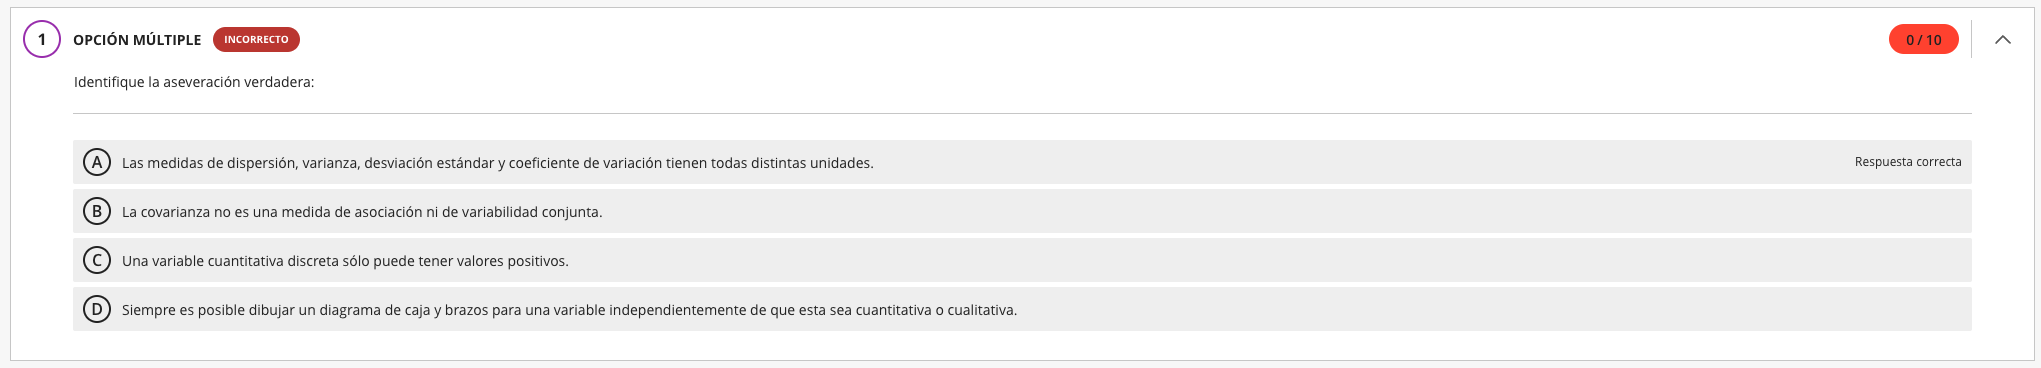
\includegraphics[width=1\textwidth]{images/pregunta1.png}
\end{figure}
\textbf{Respuesta correcta: Las medidas de dispersión, varianza, desviación estándar y coeficiente de variación tienen todas distintas unidades.}\\
Cada una de estas medidas de dispersión tiene unidades diferentes:\\
\begin{itemize}
    \item \textit{Varianza:} mide dispersión en unidades cuadradas (cuadrado).
    \item \textit{Desviación estándar:} raíz cuadrada de la varianza (base).
    \item \textit{Coeficiente de variación:} desviación estándar normalizada por la media (magnitud adimensional).
\end{itemize}
Se descartan:
\begin{itemize}
    \item \textit{"La covarianza no es una medida de asociación ni de variabilidad conjunta."}: La covarianza mide justamente como varían 2 variables conjuntamente, es una medida de asociación lineal.
    \item \textit{"Una variable cuantitativa discreta sólo puede tener valores positivos."}: Una variable discreta puede tomar tanto valores positivos como negativos.
    \item \textit{"Siempre es posible dibujar un diagrama de caja y brazos para una variable independientemente de que esta sea cuantitativa o cualitativa."}: Los boxplots requieren una variable cuantitativa por la distancia/cuartiles que usan.
\end{itemize}
%%%%%%%%%%%%%%%%%%%%%%%%%%%%%%%%%%%%%%%%%%%%%%%%%%%%
\section{Pregunta 2}
\begin{figure}[H]
    \centering
    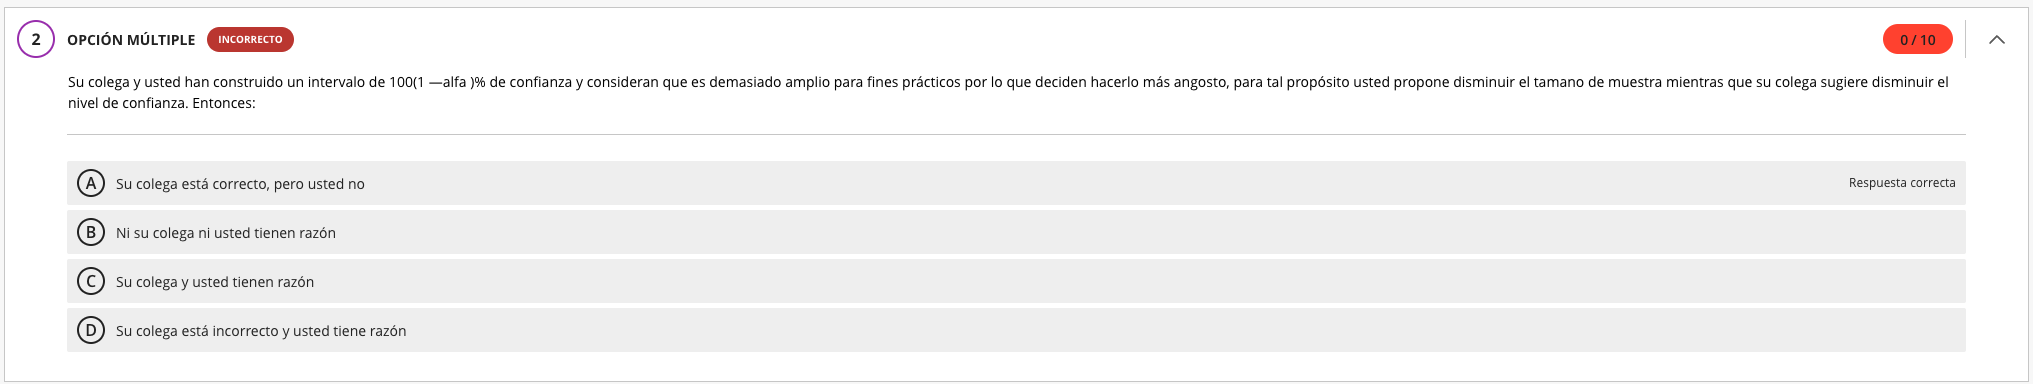
\includegraphics[width=1\textwidth]{images/pregunta2.png}
\end{figure}

\textbf{Respuesta correcta: Su colega está correcto, pero usted no.} \\ 
Para reducir un intervalo de confianza de \(100(1-\alpha)\%\) existen 2 opciones:
\begin{itemize}
    \item \emph{Disminuir el nivel de confianza} (aumentar \(\alpha\)), lo que reduce el valor crítico \(z_{1-\alpha/2}\) y por ende el margen de error.
    \item \emph{Aumentar el tamaño de muestra} \(n\), lo que disminuye el error estándar \(\sigma/\sqrt{n}\).
\end{itemize}
\textbf{Disminuir el tamaño de muestra} \emph{aumentaría} el error estándar y \emph{ampliaría} el intervalo, por lo que estamos equivocados.
En cambio, nuestro amigo propone \textbf{disminuir el nivel de confianza}, que \emph{reduce} el valor crítico y \emph{estrecha} el intervalo, por lo que él está en lo correcto.
%%%%%%%%%%%%%%%%%%%%%%%%%%%%%%%%%%%%%%%%%%%%%%%%%%%%
\section{Pregunta 3}
\begin{figure}[H]
    \centering
    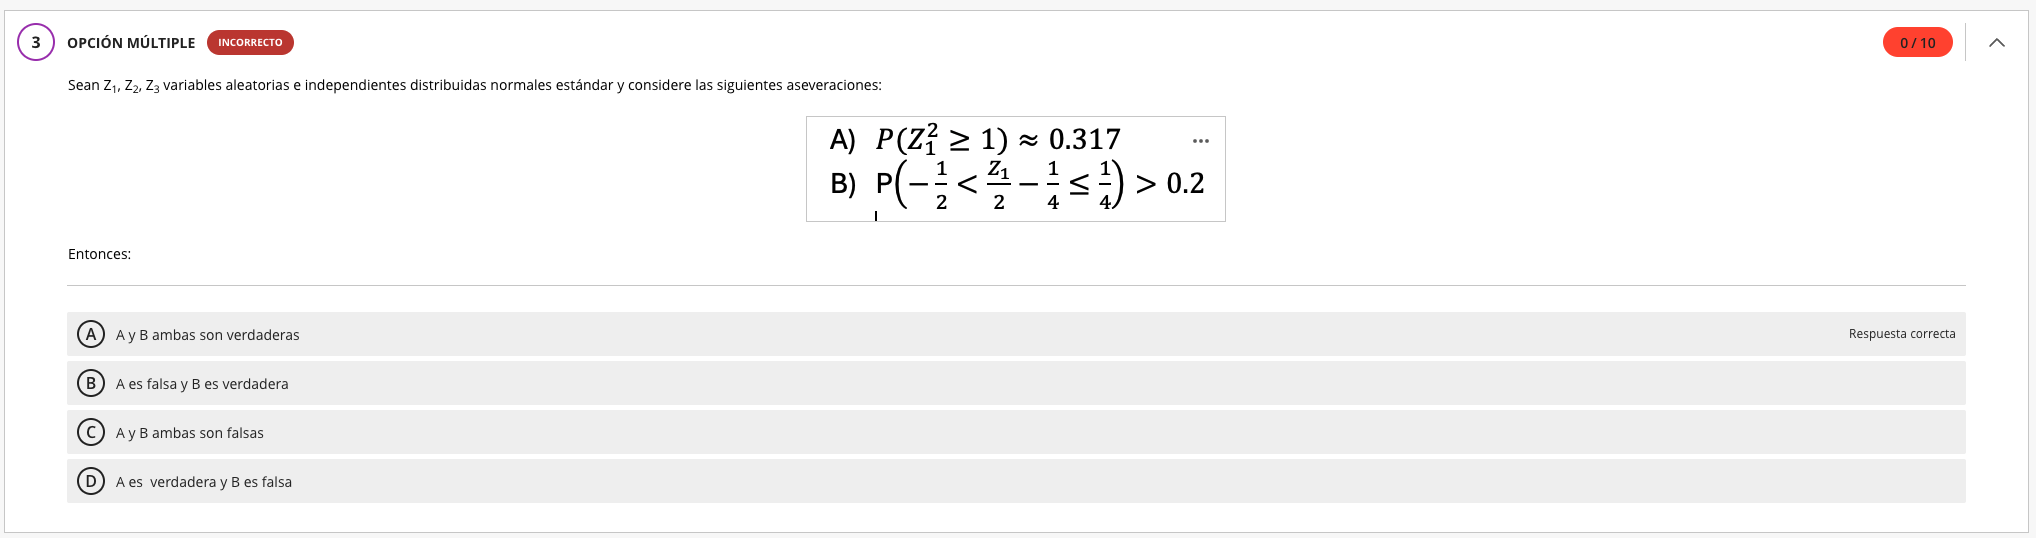
\includegraphics[width=1\textwidth]{images/pregunta3.png}
\end{figure}

\textbf{Respuesta correcta: A y B ambas son verdaderas.}  
\begin{itemize}
    \item \textit{A}: 
    \[
      P(Z_1^2 \ge 1) \;=\; P(|Z_1| \ge 1)
      \;=\; 2\bigl[1 - \Phi(1)\bigr]
      \;\approx\; 2(0.1587)
      \;\approx\; 0.3174.
    \]
    \item \textit{B}:
    \[
        \begin{aligned}
            T &= \frac{Z_1}{2} - \frac14
                  \;\sim\; N\!\bigl(\mu=-\tfrac14,\;\sigma^2=\tfrac14\bigr),\\
            P\Bigl(-\tfrac12 \le T \le \tfrac14\Bigr)
            &= P\!\Bigl(\tfrac{-\tfrac12 + \tfrac14}{0.5} \le U \le \tfrac{\tfrac14 + \tfrac14}{0.5}\Bigr)\\
            &= P\bigl(-0.5 \le U \le 1\bigr)
            = \Phi(1) - \Phi(-0.5)
            \;\approx\; 0.8413 - 0.3085
            \;\approx\; 0.5328
            > 0.2.
        \end{aligned}
    \]
\end{itemize}
%%%%%%%%%%%%%%%%%%%%%%%%%%%%%%%%%%%%%%%%%%%%%%%%%%%%
\section{Pregunta 4}
\begin{figure}[H]
    \centering
    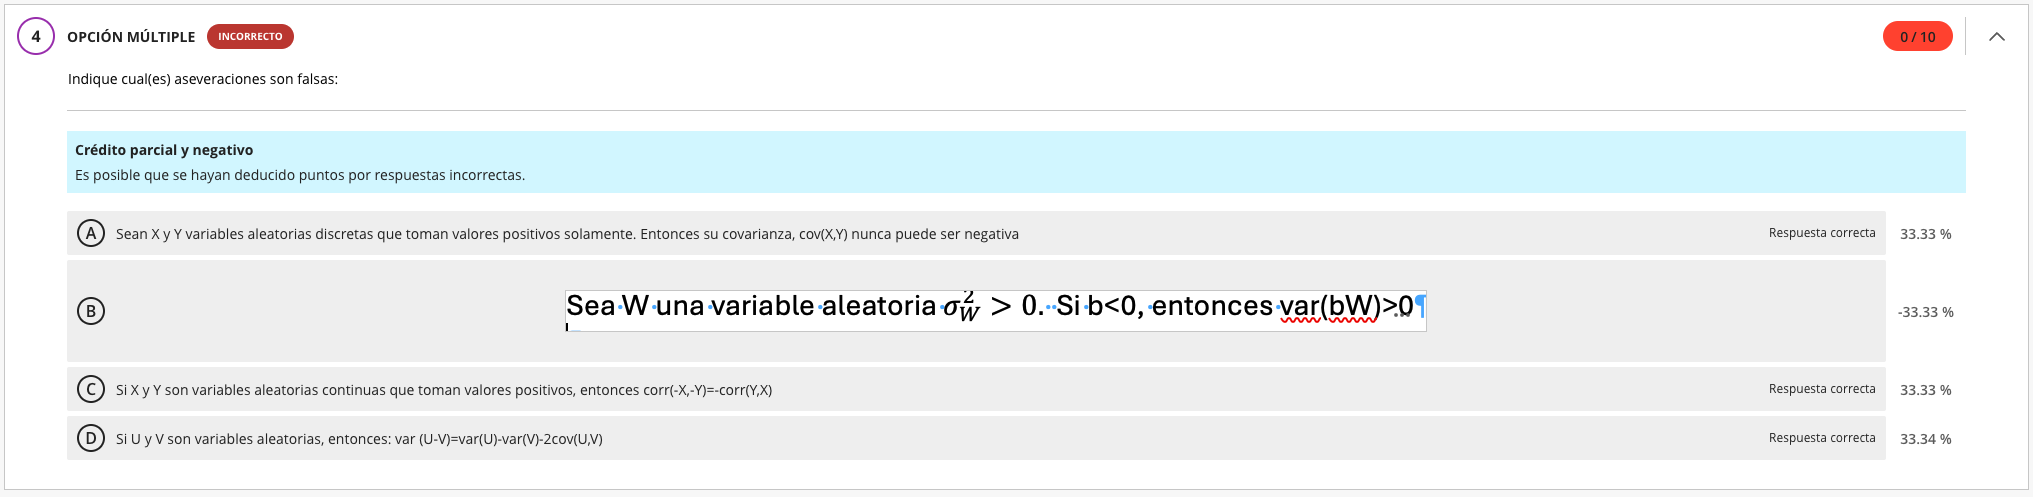
\includegraphics[width=1\textwidth]{images/pregunta4.png}
\end{figure}

\textbf{Respuesta correcta: A, C y D son falsas.}\\
Las aseveraciones A, C y D son falsas por:

\begin{itemize}
    \item \textit{"Sean X y Y variables aleatorias discretas que toman valores positivos solamente. Entonces su covarianza, cov(X,Y) nunca puede ser negativa"}: Falso, la covarianza puede ser negativa si valores altos de X se asocian con valores bajos de Y.
    \item \textit{"Si X y Y son variables aleatorias continuas que toman valores positivos, entonces corr(-X,Y)=corr(Y,X)"}: Falso  
    \[
      \corr(-X,Y)=\frac{\Cov(-X,Y)}{\sigma_X\,\sigma_Y}
      =-\frac{\Cov(X,Y)}{\sigma_X\,\sigma_Y}
      =-\corr(X,Y)
      \neq \corr(Y,X)\,.
    \]
    \item \textit{"Si U y V son variables aleatorias, entonces $var(U-V)=var(U)-var(V)-2\,\Cov(U,V)"$}:\\ Falso, la fórmula sería:  
    \[
      \Var(U-V)=\Var(U)+\Var(V)-2\,\Cov(U,V)\,.
    \]
\end{itemize}

Queda como verdadera
\begin{itemize}
    \item \textit{"Sea W una variable aleatoria \(\sigma_W^2>0\). Si \(b<0\), entonces \(\Var(bW)>0\)"}:\\ Verdadero, porque \(\Var(bW)=b^2\,\Var(W)>0\) siempre que \(\Var(W)>0\) y \(b\neq0\).
\end{itemize}
%%%%%%%%%%%%%%%%%%%%%%%%%%%%%%%%%%%%%%%%%%%%%%%%%%%%
\section{Pregunta 5}
\begin{figure}[H]
    \centering
    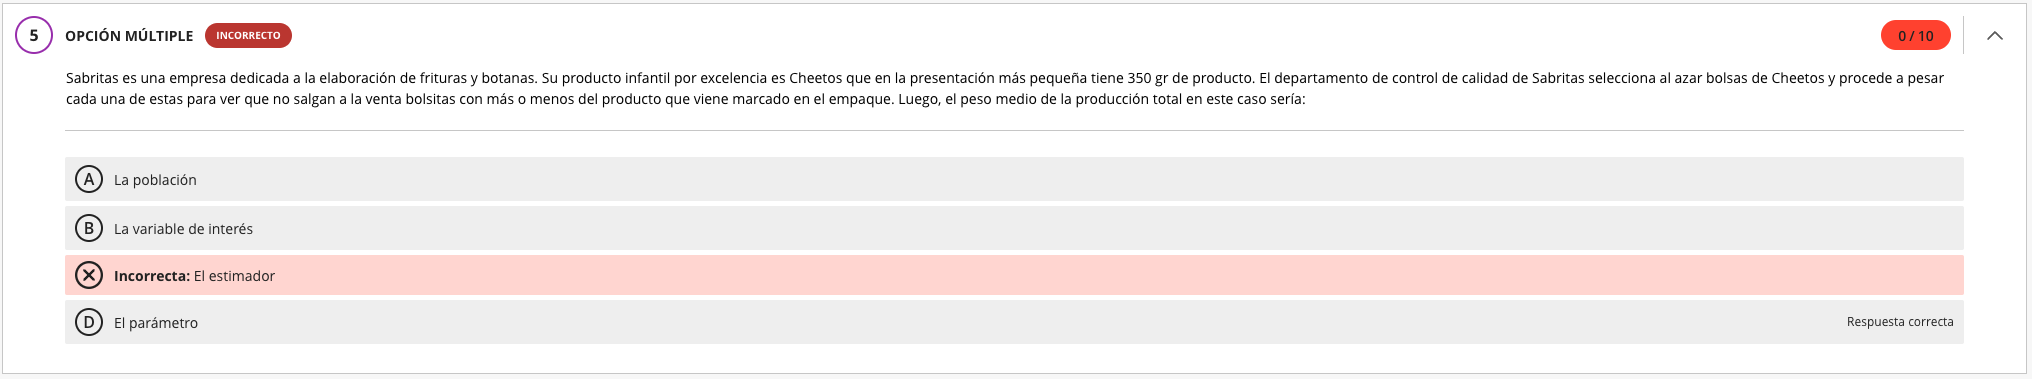
\includegraphics[width=1\textwidth]{images/pregunta5.png}
\end{figure}

\textbf{Respuesta correcta: El parámetro.}  
El peso medio de todas las bolsas de Cheetos producidas es una característica \emph{fija} de la población completa, es decir, un \textbf{parámetro} poblacional.

Se descartan:
\begin{itemize}
    \item \textit{"La población"}: conjunto de todas las bolsas, no la \emph{medida} de su peso medio.
    \item \textit{"La variable de interés"}: variable de interés, el \emph{peso} de cada bolsa, no la \emph{media} de esa variable.
    \item \textit{El Estimador}: el estimador sería la \emph{media muestral} calculada a partir de una muestra.
\end{itemize}
%%%%%%%%%%%%%%%%%%%%%%%%%%%%%%%%%%%%%%%%%%%%%%%%%%%%
\section{Pregunta 6}
\begin{figure}[H]
    \centering
    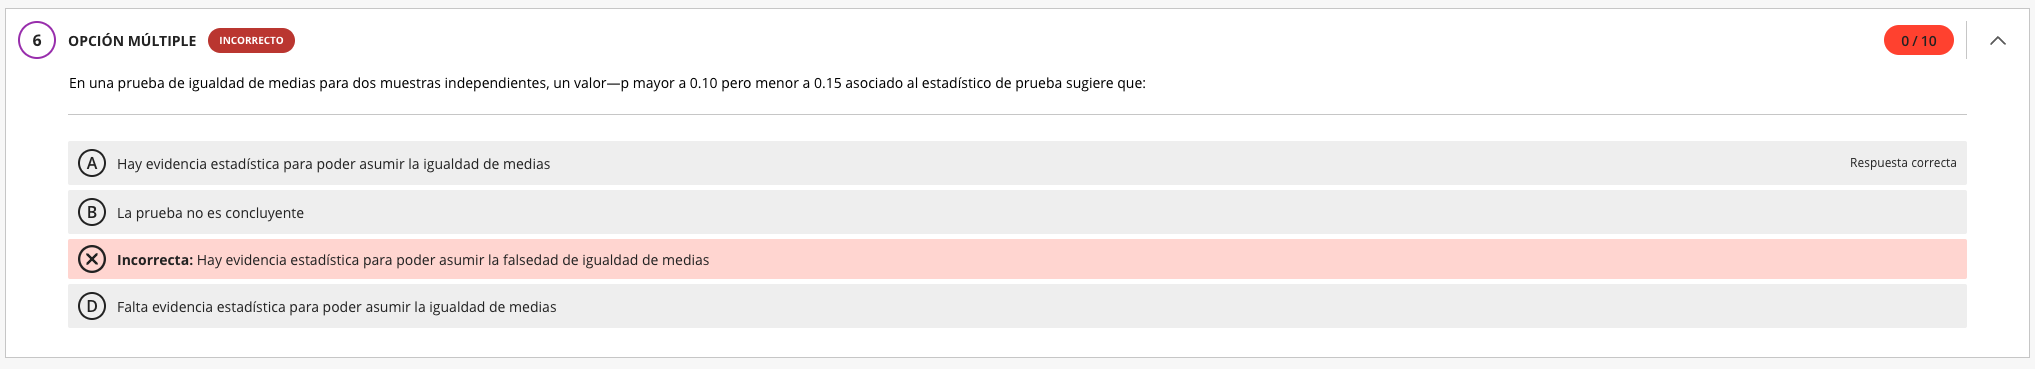
\includegraphics[width=1\textwidth]{images/pregunta6.png}
\end{figure}

\textbf{Respuesta correcta: Hay evidencia estadística para poder asumir la igualdad de medias.}  
Con un nivel de significancia \(\alpha=0.10\), si el valor-p asociado al estadístico de prueba es mayor que 0.10 (aunque menor que 0.15), no rechazamos \(H_0\). Al no encontrar evidencia contra la hipótesis nula, podemos \emph{asumir} que las medias son iguales en ese nivel de confianza.

Se descartan:
\begin{itemize}
  \item \textit{"La prueba no es concluyente"}: Aunque el p-valor esté en la “zona gris” entre 0.10 y 0.15, sigue siendo mayor que el umbral de 0.10, por lo que no se rechaza \(H_0\).
  \item \textit{"Hay evidencia estadística para poder asumir la falsedad de igualdad de medias"}: Sería falso, pues para rechazar \(H_0\) necesitaríamos \(p\le0.10\).
  \item \textit{"Falta evidencia estadística para poder asumir la igualdad de medias"}: Equivocado, porque al no rechazar \(H_0\) ya tenemos evidencia suficiente para asumir la igualdad en ese nivel de confianza.
\end{itemize}
%%%%%%%%%%%%%%%%%%%%%%%%%%%%%%%%%%%%%%%%%%%%%%%%%%%%
\section{Pregunta 7}
\begin{figure}[H]
    \centering
    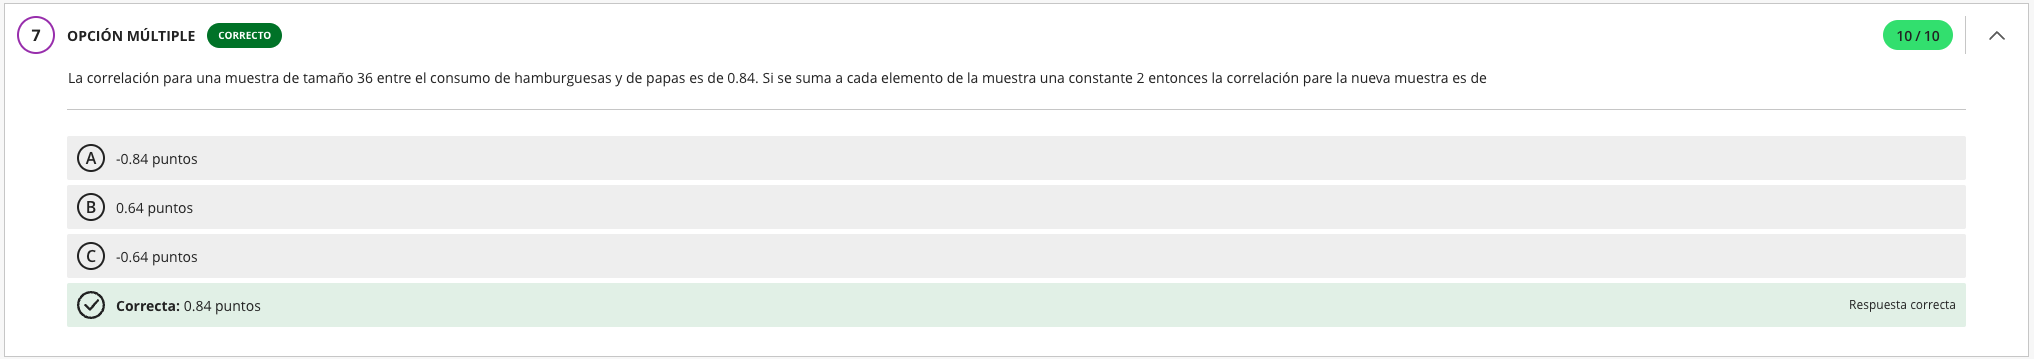
\includegraphics[width=1\textwidth]{images/pregunta7.png}
\end{figure}

\textbf{Respuesta correcta: 0.84 puntos.} \\
La correlación muestral es invariante ante traslaciones de las variables y ante escalados positivos. Cuando sumamos 2 unidades a cada observación, la covarianza y las desviaciones estándar cambian, pero su cociente (la correlación) se mantiene igual.

Se descartan:
\begin{itemize}
    \item \textit{"-0.84 puntos"}: sumar constantes no invierte el signo de la correlación, solo un factor negativo lo afecta.
    \item \textit{"0.64 puntos"}: no hay cambio de magnitud, ya que no se multiplica por un factor distinto de 1.
    \item \textit{"-0.64 puntos"}: no aplica ni inversión de signo, ni cambio de magnitud.
\end{itemize}
%%%%%%%%%%%%%%%%%%%%%%%%%%%%%%%%%%%%%%%%%%%%%%%%%%%%
\section{Pregunta 8}
\begin{figure}[H]
    \centering
    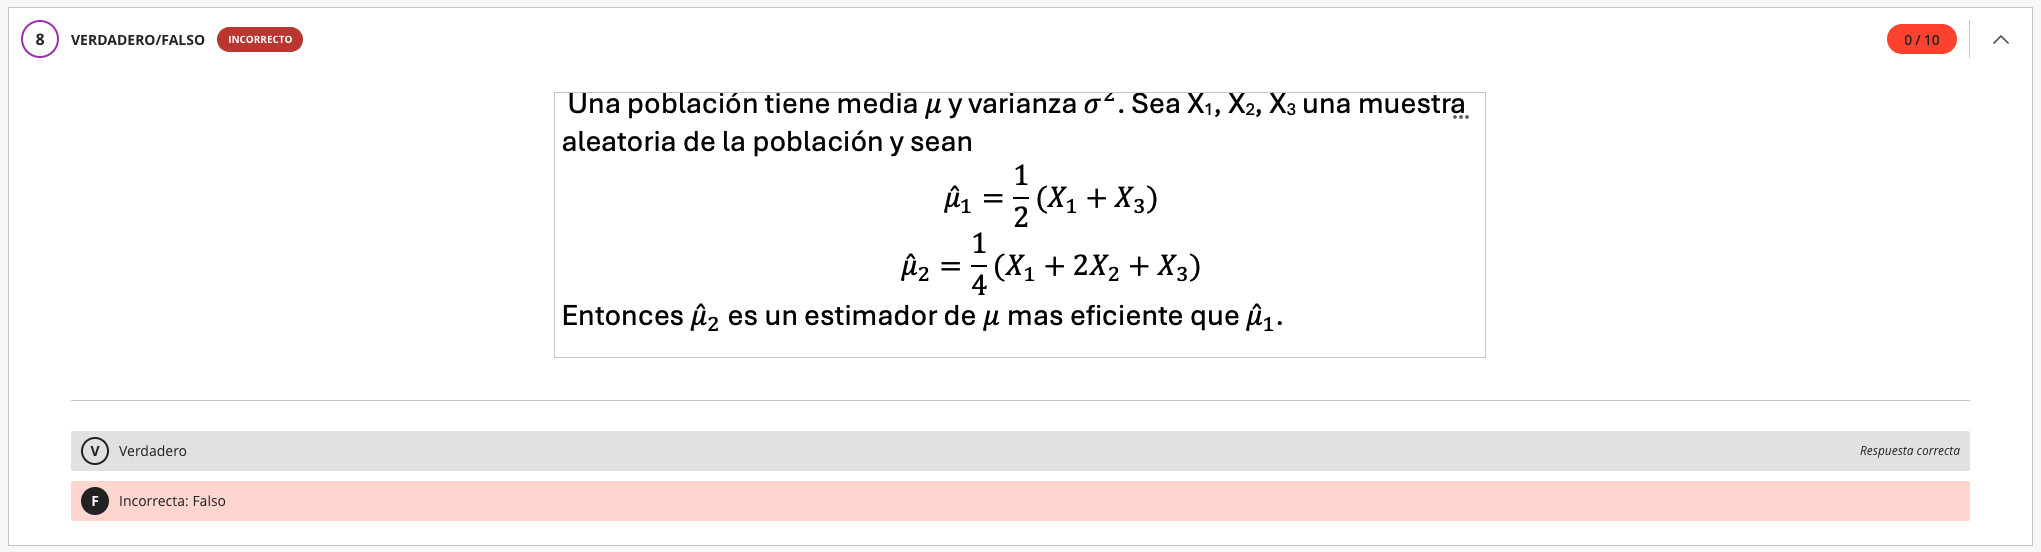
\includegraphics[width=1\textwidth]{images/pregunta8.png}
\end{figure}

\textbf{Respuesta correcta: Verdadero.} \\ 
Ambos \(\hat\mu_1\) y \(\hat\mu_2\) son \emph{no sesgados} para \(\mu\). La eficiencia se compara a través de sus varianzas:

\[
\Var(\hat\mu_1)
= \Var\!\Bigl(\tfrac{1}{2}(X_1 + X_3)\Bigr)
= \tfrac{1}{4}\bigl[\Var(X_1)+\Var(X_3)\bigr]
= \tfrac{1}{4}(2\sigma^2)
= \tfrac{1}{2}\,\sigma^2.
\]

\[
\Var(\hat\mu_2)
= \Var\!\Bigl(\tfrac{1}{4}(X_1 + 2X_2 + X_3)\Bigr)
= \tfrac{1}{16}\bigl[\Var(X_1)+4\Var(X_2)+\Var(X_3)\bigr]
= \tfrac{1}{16}(6\sigma^2)
= \tfrac{3}{8}\,\sigma^2.
\]

Como 
\(\tfrac{3}{8}\sigma^2 < \tfrac{1}{2}\sigma^2\),
\(\hat\mu_2\) tiene menor varianza y por tanto es más eficiente que \(\hat\mu_1\).
%%%%%%%%%%%%%%%%%%%%%%%%%%%%%%%%%%%%%%%%%%%%%%%%%%%%
\section{Pregunta 9}
\begin{figure}[H]
    \centering
    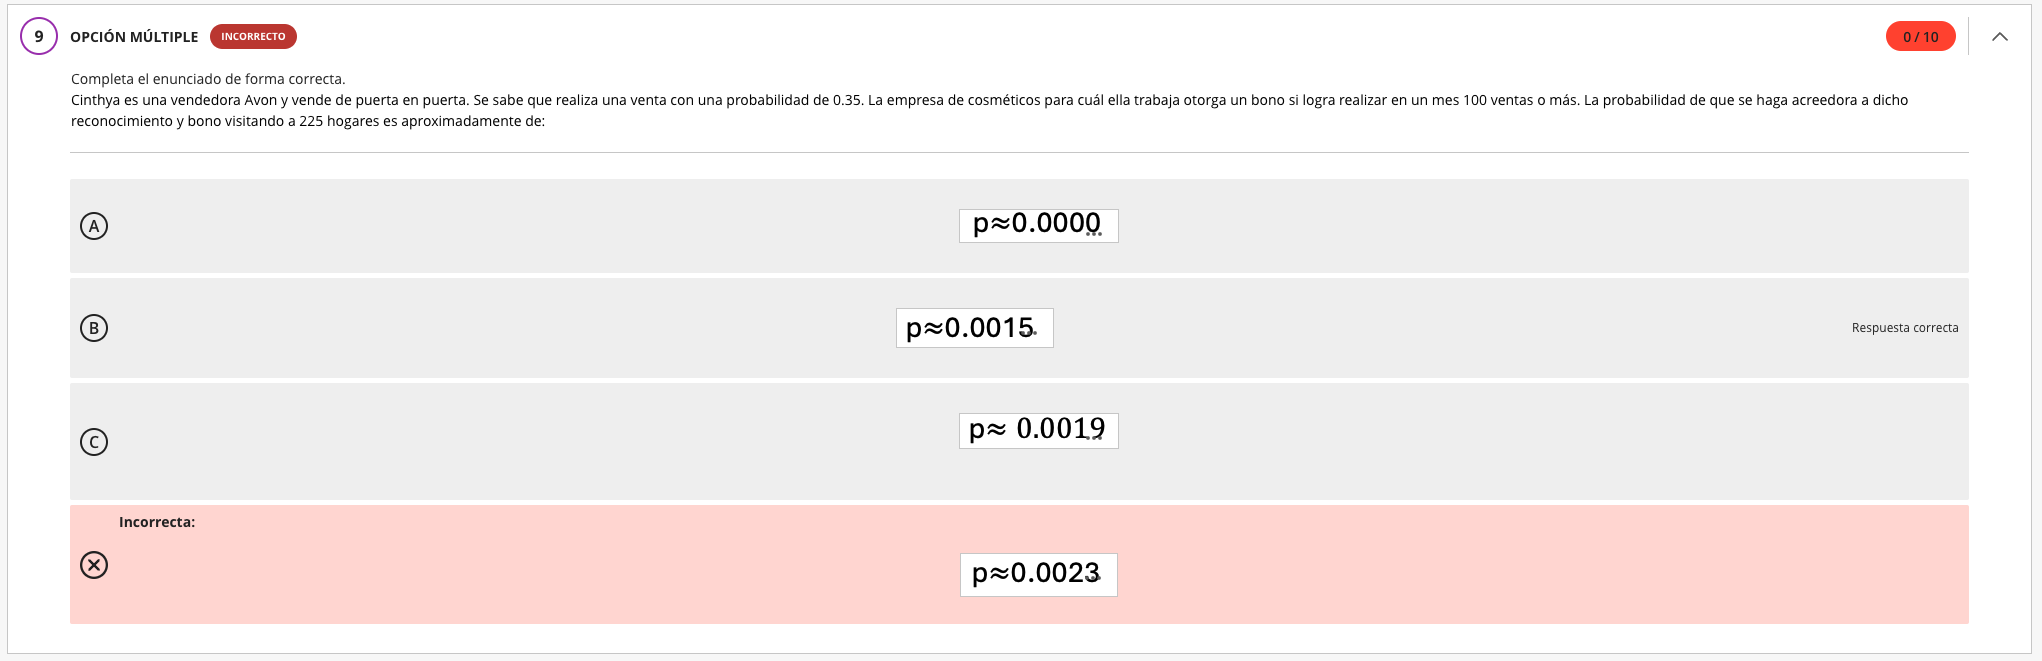
\includegraphics[width=1\textwidth]{images/pregunta9.png}
\end{figure}

\textbf{Respuesta correcta: \(p \approx 0.0015\).} \\ 
Sea \(X\sim \mathrm{Bin}(n=225,\;p=0.35)\). Buscamos  
\[
P(X \ge 100).
\]  
Usando la aproximación normal sin corrección de continuidad:
\[
\mu = np = 225 \times 0.35 = 78.75,\qquad
\sigma = \sqrt{np(1-p)} = \sqrt{78.75 \times 0.65}\approx 7.15.
\]
Entonces
\[
Z = \frac{100 - 78.75}{7.15} \approx 2.97,
\]
y
\[
P(X\ge100)\approx 1 - \Phi(2.97) \approx 0.0015.
\]
%%%%%%%%%%%%%%%%%%%%%%%%%%%%%%%%%%%%%%%%%%%%%%%%%%%%
\section{Pregunta 10}
\begin{figure}[H]
    \centering
    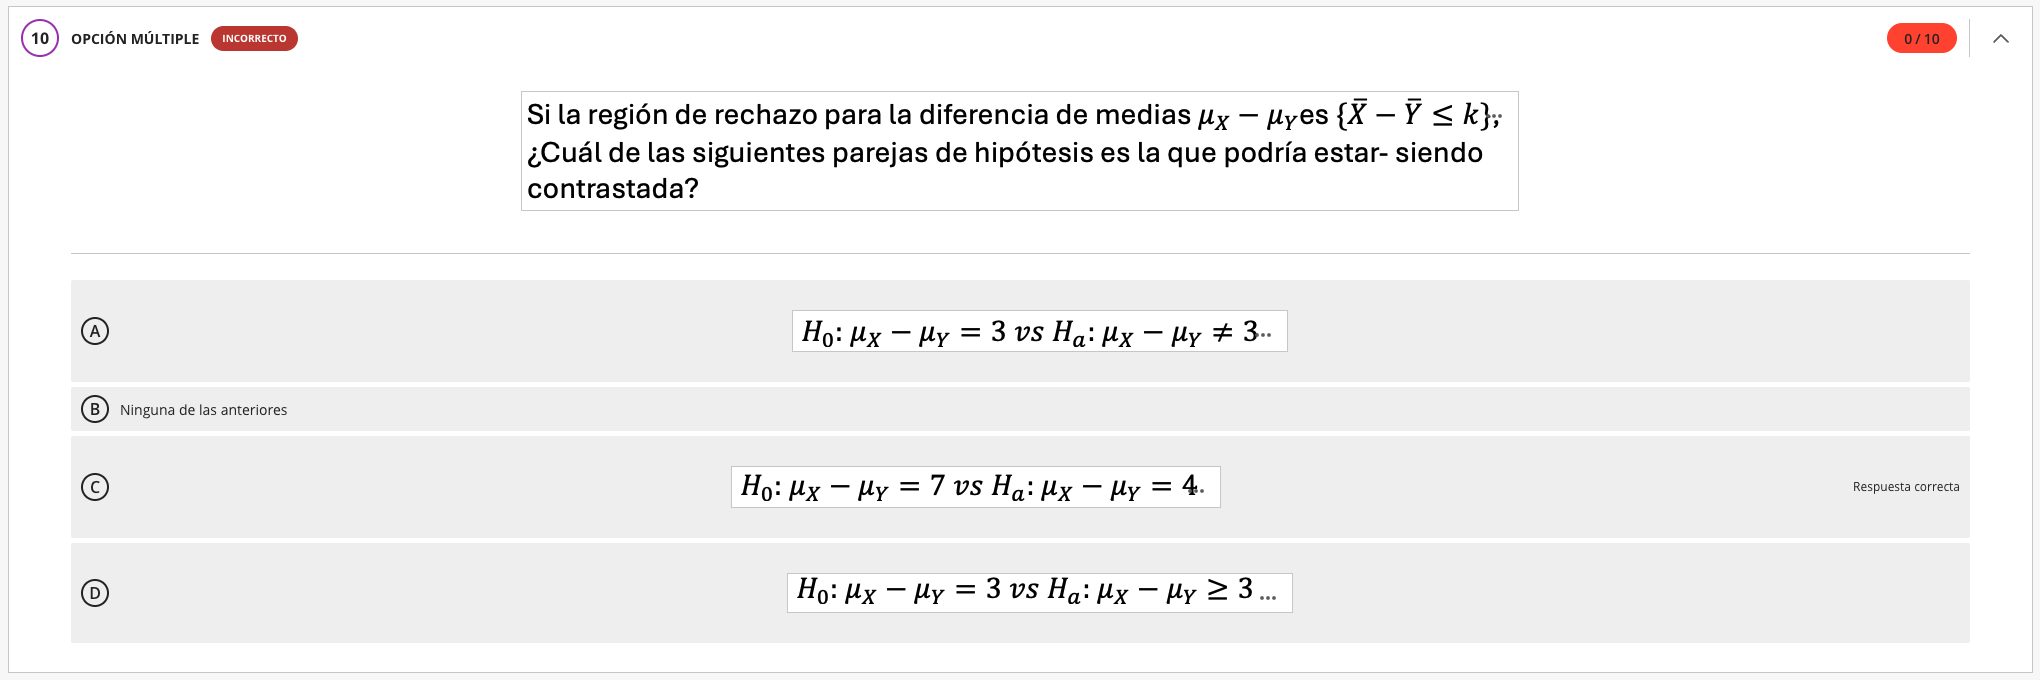
\includegraphics[width=1\textwidth]{images/pregunta10.png}
\end{figure}

\textbf{Respuesta correcta: \(H_0: \mu_X - \mu_Y = 7\) vs. \(H_a: \mu_X - \mu_Y < 4\).}  \\
La región de rechazo \(\{\bar X - \bar Y \le k\}\) resulta de un test de una cola a la izquierda, donde se rechaza la igualdad de medias si la diferencia muestral es suficientemente pequeña.  

Se descartan:
\begin{itemize}
  \item \textit{"\(H_0: \mu_X - \mu_Y = 3\) vs. \(H_a: \mu_X - \mu_Y \neq 3\)"}: es un test bilateral, no cuadra con una sola cola.  
  \item \textit{"\(H_0: \mu_X - \mu_Y = 3\) vs. \(H_a: \mu_X - \mu_Y \ge 3\)"}: ese sería un test de cola derecha (rechaza por valores grandes), al contrario del enunciado.
\end{itemize}
%%%%%%%%%%%%%%%%%%%%%%%%%%%%%%%%%%%%%%%%%%%%%%%%%%%%
\end{document}
